\chapter{Logistic Regression}
\label{chap:logistic_regression}

\section{Introduction}
Logistic Regression is a fundamental \textbf{Supervised Learning} algorithm used for \textbf{Classification} problems.
\begin{definition}
\textbf{Classification} is the task of predicting discrete class labels (e.g., Yes/No, Spam/Not Spam) rather than continuous values.
\end{definition}

\subsection{Story: The Medical Diagnosis}
Imagine a doctor trying to determine if a tumor is \textbf{Malignant} (Cancerous, Class 1) or \textbf{Benign} (Safe, Class 0) based on its \textbf{Size}.
\begin{itemize}
    \item \textbf{Linear Regression approach}: If we fit a straight line, it might predict a value of 0.8 for small tumors, but 1.5 or 2.0 for large tumors.
    \item \textbf{Problem}: What does a value of 2.0 mean? Can probability be $> 100\%$? No.
    \item \textbf{Solution}: We need a function that bounds the output between 0 and 1.
\end{itemize}
This is where Logistic Regression comes in. It predicts the \textbf{Probability} that a given instance belongs to Class 1.

\section{Geometric Intuition}
Geometrically, Logistic Regression tries to find a \textbf{Linear Decision Boundary} that separates the two classes in space.

\begin{figure}[htbp]
\centering
\begin{tikzpicture}
    \begin{axis}[
        xlabel={$x_1$},
        ylabel={$x_2$},
        axis lines=middle,
        width=0.7\textwidth,
        height=0.7\textwidth,
        xtick=\empty, ytick=\empty
    ]
    % Class 0 (Blue Circles)
    \addplot[only marks, mark=o, color=blue] coordinates {
        (1, 1) (1.5, 2) (2, 1) (2, 2.5) (3, 1.5)
    };
    \addlegendentry{Class 0}
    
    % Class 1 (Red Squares)
    \addplot[only marks, mark=square*, color=red] coordinates {
        (4, 4) (4.5, 5) (5, 3.5) (5.5, 4.5) (6, 4)
    };
    \addlegendentry{Class 1}
    
    % Decision Boundary
    \addplot[domain=0:6, color=black, thick, dashed] {-x + 5.5};
    \node[right] at (axis cs:0, 5.5) {Decision Boundary ($w^T x + b = 0$)};
    \end{axis}
\end{tikzpicture}
\caption{Geometric View: Finding a line that separates Blue circles from Red squares.}
\label{fig:log_reg_geometry}
\end{figure}

The equation of this boundary is:
\begin{equation}
    z = w \cdot x + b = w_1 x_1 + \dots + w_n x_n + b
\end{equation}
\begin{itemize}
    \item If $z > 0$, the point is on the ``Positive'' side $\rightarrow$ Predict Class 1.
    \item If $z < 0$, the point is on the ``Negative'' side $\rightarrow$ Predict Class 0.
\end{itemize}

\section{The Sigmoid Function}
We computed $z$ (the distance from the boundary). Now we need to convert this $z$ ($-\infty$ to $+\infty$) into a Probability ($0$ to $1$).
We use the \textbf{Sigmoid Function} (also called the Logistic Function):
\begin{equation}
    \sigma(z) = \frac{1}{1 + e^{-z}}
\end{equation}

\begin{figure}[htbp]
\centering
\begin{tikzpicture}
    \begin{axis}[
        xlabel={$z$ ($w \cdot x + b$)},
        ylabel={$\sigma(z)$ (Probability)},
        xmin=-6, xmax=6,
        ymin=0, ymax=1.1,
        axis lines=middle,
        grid=major,
        width=0.8\textwidth,
        height=0.5\textwidth
    ]
    \addplot[domain=-6:6, color=blue, uber thick, samples=100] {1/(1+exp(-x))};
    \draw[dashed] (axis cs:-6, 0.5) -- (axis cs:6, 0.5);
    \node[above] at (axis cs:-4, 0.5) {Threshold (0.5)};
    \end{axis}
\end{tikzpicture}
\caption{The Sigmoid Function: Squashing any number into range $[0, 1]$.}
\label{fig:sigmoid}
\end{figure}

\textbf{Properties}:
\begin{itemize}
    \item When $z = 0$, $\sigma(z) = 0.5$ (The Decision Boundary).
    \item When $z \to +\infty$ (deep in positive territory), $\sigma(z) \to 1$.
    \item When $z \to -\infty$ (deep in negative territory), $\sigma(z) \to 0$.
\end{itemize}


\section{Loss Function: Why not MSE?}
In Linear Regression, we used Mean Squared Error (MSE). Can we use it here?
\begin{equation}
    J = \frac{1}{n} \sum (\sigma(z) - y)^2
\end{equation}
If you plot this loss function against weights ($w$) for a Sigmoid model, it turns out to be \textbf{Non-Convex}. It looks like a wavy surface with many "Local Minima" (valleys that aren't the deepest). Gradient Descent would get stuck in these valleys.

\begin{figure}[htbp]
\centering
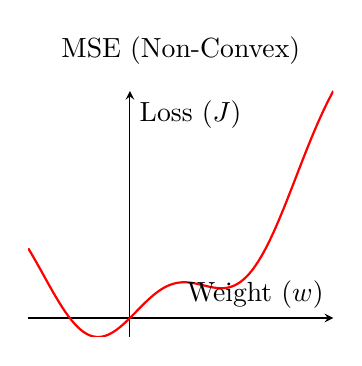
\begin{tikzpicture}
    \begin{axis}[
        xlabel={Weight ($w$)},
        ylabel={Loss ($J$)},
        ticks=none,
        axis lines=middle,
        width=0.45\textwidth,
        title={MSE (Non-Convex)}
    ]
    \addplot[domain=-2:4, samples=100, smooth, thick, color=red] {sin(deg(x*2)) + 0.5*x^2};
    \end{axis}
\end{tikzpicture}
\hfill
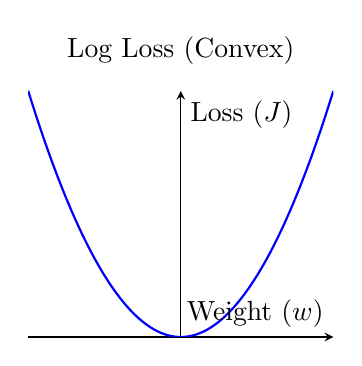
\begin{tikzpicture}
    \begin{axis}[
        xlabel={Weight ($w$)},
        ylabel={Loss ($J$)},
        ticks=none,
        axis lines=middle,
        width=0.45\textwidth,
        title={Log Loss (Convex)}
    ]
    \addplot[domain=-2:2, samples=100, smooth, thick, color=blue] {x^2};
    \end{axis}
\end{tikzpicture}
\caption{MSE creates a wavy surface (left) where GD gets stuck. Log Loss creates a smooth bowl (right).}
\label{fig:convex_vs_nonconvex}
\end{figure}

\section{Maximum Likelihood Estimation (MLE)}
Instead of minimizing error, we change our perspective. We want to find the weights $w$ that \textbf{Maximize the Likelihood} of observing our data.
\begin{itemize}
    \item If $y=1$, we want $\hat{y}$ (probability) to be close to 1.
    \item If $y=0$, we want $\hat{y}$ to be close to 0 (or $1-\hat{y}$ close to 1).
\end{itemize}
Combining these, we derive the **Binary Cross Entropy** (Log Loss) function:
\begin{equation}
    J(w) = - \frac{1}{n} \sum_{i=1}^{n} [ y_i \log(\hat{y}_i) + (1-y_i) \log(1 - \hat{y}_i) ]
\end{equation}
This function is \textbf{Convex} (smooth bowl), ensuring Gradient Descent always finds the global optimum.

\section{Gradient Descent Derivation}
We need to update weights: $w_{new} = w_{old} - \eta \frac{\partial J}{\partial w}$.
Using the Chain Rule:
\begin{equation}
    \frac{\partial J}{\partial w} = \frac{\partial J}{\partial \hat{y}} \cdot \frac{\partial \hat{y}}{\partial z} \cdot \frac{\partial z}{\partial w}
\end{equation}
After some calculus (which simplifies beautifully), we get:
\begin{equation}
    \frac{\partial J}{\partial w} = \frac{1}{n} X^T (\hat{Y} - Y)
\end{equation}
\textbf{Surprise}: This is the \textit{exact same formula} as Linear Regression!
\begin{itemize}
    \item Linear Regression: $\hat{Y} = Xw$
    \item Logistic Regression: $\hat{Y} = \sigma(Xw)$
\end{itemize}
This elegance is why these algorithms are so fundamental.


\section{Evaluation Metrics}
Accuracy ($\frac{Correct}{Total}$) is often misleading, especially with imbalanced data (e.g., 99\% healthy, 1\% cancer). A model that predicts "Healthy" for everyone has 99\% accuracy but is useless.

\subsection{Confusion Matrix}
\begin{table}[htbp]
    \centering
    \begin{tabular}{|l|l|l|}
    \hline
    & \textbf{Predicted Positive (1)} & \textbf{Predicted Negative (0)} \\ \hline
    \textbf{Actual Positive (1)} & True Positive (TP) & False Negative (FN) \\ \hline
    \textbf{Actual Negative (0)} & False Positive (FP) & True Negative (TN) \\ \hline
    \end{tabular}
    \caption{Confusion Matrix: The 4 outcomes of prediction.}
\end{table}

\subsection{Precision vs Recall: The Tradeoff}
\begin{itemize}
    \item \textbf{Precision} (``Don't Spam Me''): Out of all claimed Positives, how many are real?
    \begin{equation}
        \text{Precision} = \frac{TP}{TP + FP}
    \end{equation}
    \textit{Scenario}: **Spam Filter**. A False Positive (Job Offer marked as Spam) is disastrous. We want High Precision.

    \item \textbf{Recall} (``Don't Miss It''): Out of all actual Positives, how many did we find?
    \begin{equation}
        \text{Recall} = \frac{TP}{TP + FN}
    \end{equation}
    \textit{Scenario}: **Cancer Detection**. A False Negative (Sick patient told they are healthy) is fatal. We want High Recall.
\end{itemize}

\subsection{F1 Score}
If we need a balance, we use the Harmonic Mean of Precision and Recall.
\begin{equation}
    \text{F1} = 2 \cdot \frac{P \cdot R}{P + R}
\end{equation}
Why Harmonic Mean? Because it punishes extreme values. If Recall is 0, F1 becomes 0 (Arithmetic mean would say 0.5).

\textbf{HOTS Question}: Which is worse, Type I (FP) or Type II (FN) error?
\\ \textit{Answer: It depends on the business problem! For Cancer, Type II is worse. For Spam, Type I is worse.}

\section{Multiclass Classification}
What if we have 3 classes: Dog, Cat, Rabbit?

\subsection{Strategy 1: One-Vs-Rest (OvR)}
We train 3 separate binary classifiers:
\begin{enumerate}
    \item Dog vs [Cat, Rabbit]
    \item Cat vs [Dog, Rabbit]
    \item Rabbit vs [Dog, Cat]
\end{enumerate}
The classifier with the highest probability wins.

\subsection{Strategy 2: Softmax Regression}
Generalization of Logistic Regression. We replace the Sigmoid function with the \textbf{Softmax Function}, which normalizes $K$ scores into a probability distribution summing to 1.
\begin{equation}
    P(y=j|x) = \frac{e^{z_j}}{\sum_{k=1}^{K} e^{z_k}}
\end{equation}
When using Softmax, the loss function is \textbf{Categorical Cross Entropy}.

\subsection{Metrics for Multiclass}
\begin{itemize}
    \item \textbf{Macro Average}: Calculate F1 for each class (Dog, Cat, Rabbit) and simple average them. Treats all classes equally.
    \item \textbf{Weighted Average}: Weight the average by the number of samples in each class. Better for imbalanced data.
\end{itemize}


\section{Handling Non-Linear Data}
Standard Logistic Regression creates a linear decision boundary (Line/Hyperplane). It fails if classes are separated by a circle or curve.

\subsection{Polynomial Features}
We can solve this by creating \textbf{Polynomial Features} (e.g., $x^2, x^3$).
\begin{equation}
    z = w_1 x + w_2 x^2 + b
\end{equation}
The model still sees this as linear (in terms of weights), but in the original 2D space, it draws a curve (Parabola/Circle).

\subsection{Implementation}
Use `PolynomialFeatures` in a Pipeline.
\begin{lstlisting}[language=Python]
from sklearn.preprocessing import PolynomialFeatures
from sklearn.pipeline import Pipeline

model = Pipeline([
    ('poly', PolynomialFeatures(degree=3)),
    ('log_reg', LogisticRegression())
])
model.fit(X, y)
\end{lstlisting}

\section{Implementation in Python}
Let's predict whether a user purchases a product (1) or not (0) based on Age and Salary.

\begin{lstlisting}[language=Python, caption=Logistic Regression Step-by-Step]
import numpy as np
from sklearn.model_selection import train_test_split
from sklearn.preprocessing import StandardScaler
from sklearn.linear_model import LogisticRegression
from sklearn.metrics import classification_report

# Step 1: Create Dummy Data (Age, Salary)
# 100 people.
X = np.random.rand(100, 2) * [50, 50000] + [20, 30000] # Age 20-70, Salary 30k-80k
# Purchase if Age > 40 OR Salary > 60k
y = ((X[:, 0] > 40) | (X[:, 1] > 60000)).astype(int)

# Step 2: Split
X_train, X_test, y_train, y_test = train_test_split(X, y, test_size=0.2, random_state=42)

# Step 3: Scaling (CRITICAL for Logistic Regression)
# GD converges faster if features are on same scale (e.g. -1 to 1).
scaler = StandardScaler()
X_train_scaled = scaler.fit_transform(X_train)
X_test_scaled = scaler.transform(X_test)

# Step 4: Train
model = LogisticRegression(random_state=42)
model.fit(X_train_scaled, y_train)

# Step 5: Evaluate
y_pred = model.predict(X_test_scaled)
print(classification_report(y_test, y_pred, target_names=['Not Purchased', 'Purchased']))
\end{lstlisting}

\section{Key Takeaways}
\begin{itemize}
    \item \textbf{Probability Output}: Unlike Linear Regression, it outputs a probability (0 to 1) using the \textbf{Sigmoid} function.
    \item \textbf{Decision Boundary}: It finds a linear line/hyperplane to separate classes.
    \item \textbf{Log Loss}: The convex loss function derived from Maximum Likelihood Estimation.
    \item \textbf{Precision vs Recall}: Choose based on the cost of error (Spam vs Cancer).
    \item \textbf{Scaling}: Always scale features before training Logistic Regression.
\end{itemize}


